
% This LaTeX was auto-generated from MATLAB code.
% To make changes, update the MATLAB code and republish this document.











    
    \begin{DoxyCode}
function example_dirac_adjoint()
\end{DoxyCode}
\begin{par}
COMPILATION
\end{par} \vspace{1em}
\begin{DoxyCode}
    [exdir,~,~]=fileparts(which('example_dirac_adjoint.m'));
    % compile the model
    amiwrap('model_dirac_adjoint','model_dirac_adjoint_syms',exdir)
\end{DoxyCode}

         \begin{DoxyCode}Generating model struct ...
Parsing model struct ...

Generating C code ...
headers | wrapfunctions | 
Compiling mex file ...
amici | Building with 'Xcode with Clang'.
MEX completed successfully.
Building with 'Xcode with Clang'.
MEX completed successfully.
\end{DoxyCode} 
    \begin{par}
SIMULATION
\end{par} \vspace{1em}
\begin{DoxyCode}
    % time vector
    tout = linspace(0,4,9);
    tfine = linspace(0,4,10001);
    p = [1;0.4;2;3];
    k = [];

    D.Y = [  0.00714742903826096
        -0.00204966058299775
        0.382159034587845
        0.33298932672138
        0.226111476113441
        0.147028440865854
        0.0882468698791813
        0.0375887796628869
        0.0373422340295005];

    D.Sigma_Y = 0.01*ones(size(D.Y));


    options.sensi = 1;
    options.sensi_meth = 'adjoint';
    options.maxsteps = 1e5;
    sol = simulate_model_dirac_adjoint(tout,log10(p),k,D,options);
    options.sensi = 0;
    solfine = simulate_model_dirac_adjoint(tfine,log10(p),k,[],options);
    figure
    errorbar(tout,D.Y,D.Sigma_Y)
    hold on
    plot(tfine,solfine.y)
    legend('data','simulation')
    xlabel('time t')
    ylabel('observable')
    title(['log-likelihood: ' num2str(sol.llh) ])
\end{DoxyCode}

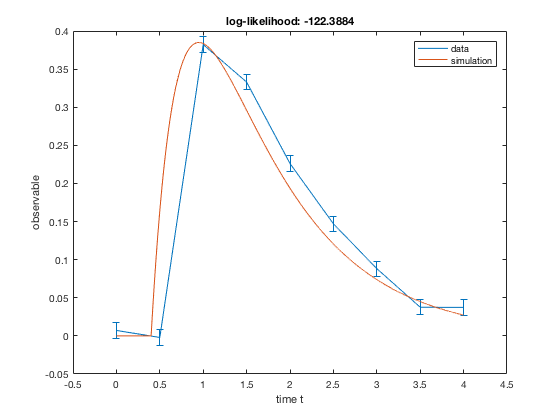
\includegraphics[width=\textwidth]{../../examples/example_dirac_adjoint/html/example_dirac_adjoint_01.png}
\begin{par}
FD
\end{par} \vspace{1em}
\begin{DoxyCode}
    eps = 1e-4;
    xi = log10(p);
    grad_fd_f = NaN(4,1);
    grad_fd_b = NaN(4,1);
    for ip = 1:4;
        options.sensi = 0;
        xip = xi;
        xip(ip) = xip(ip) + eps;
        solpf = simulate_model_dirac_adjoint(tout,xip,k,D,options);
        grad_fd_f(ip,1) = (solpf.llh-sol.llh)/eps;
        xip = xi;
        xip(ip) = xip(ip) - eps;
        solpb = simulate_model_dirac_adjoint(tout,xip,k,D,options);
        grad_fd_b(ip,1) = -(solpb.llh-sol.llh)/eps;
    end

    figure
    plot(abs(grad_fd_f),abs(sol.sllh),'o')
    hold on
    plot(abs(grad_fd_b),abs(sol.sllh),'o')
    set(gca,'XScale','log')
    set(gca,'YScale','log')
    hold on
    axis square
    plot([1e2,1e4],[1e2,1e4],'k:')
    xlim([1e2,1e4])
    ylim([1e2,1e4])
    legend('forward FD','backward FD','Location','SouthEast')
    xlabel('adjoint sensitivity absolute value of gradient element')
    ylabel('computed absolute value of gradient element')
    set(gcf,'Position',[100 300 1200 500])

    drawnow
\end{DoxyCode}

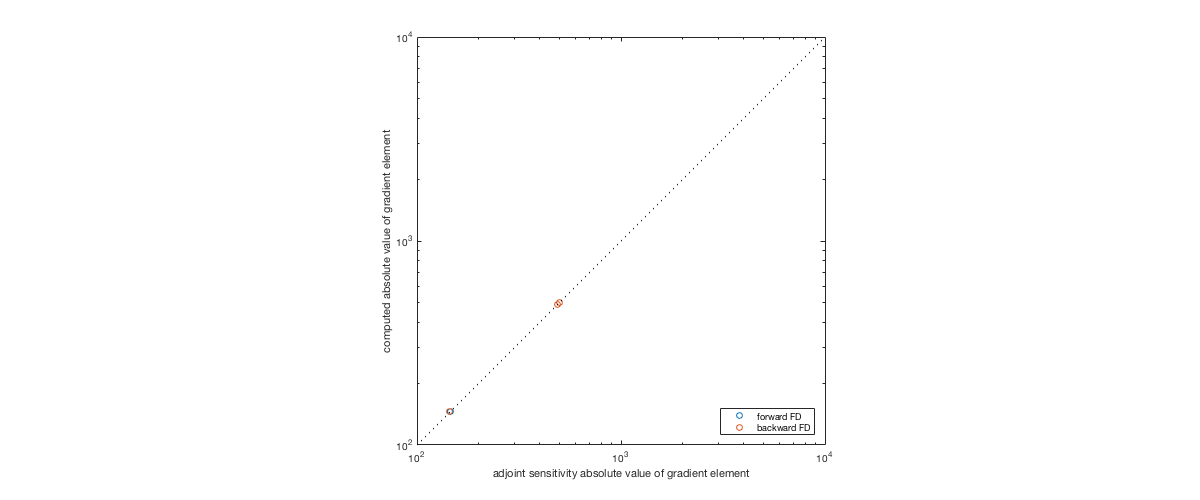
\includegraphics[width=\textwidth]{../../examples/example_dirac_adjoint/html/example_dirac_adjoint_02.png}
\begin{DoxyCode}
end
\end{DoxyCode}




    